% !TEX root = QlockToo.tex
% Kapitelvorlage

\section{Funktionen}
\label{sec:Funktionen}

\begin{multicols}{2}

Neben der Darstellung der Uhrzeit in Worten verfügt die entwickelte Wortuhr über zahlreiche weitere Funktionen. Während einige Funktionen und Modi bzw. Demonstrationsmuster nur über die Software ausgewählt werden können, so besteht für die wichtigsten Funktionen die Möglichkeit, diese über vier Taster, welche sich seitlich am Rahmen befinden, auszuwählen. Die Modi, welche über die Software auf die Uhr übertragen werden können, sind im Kapitel~\ref{sec:Software} beschreiben. Zur Übertragung muss die Uhr über die USB~-~Schnittstelle direkt an einen PC angeschlossen sein. 

 \textbf{Tasterbelegung}
 
 Über die Taster kann die Anzeige der Wortuhr wie folgt geändert werden:
\begin{description}
\item[Taster 1] Anzeige der Uhrzeit in Worten.
\end {description}
{
\centering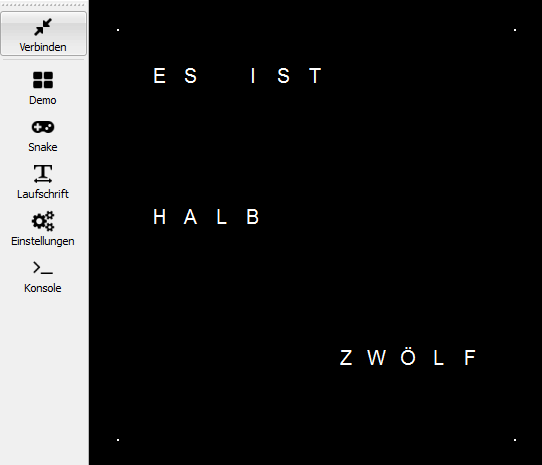
\includegraphics[width=0.8\columnwidth]{Abbildungen/Funktionen/Uhrzeit_01}

}

\begin{description}
\item[Taster 2] Anzeige der Sekunden.
\end {description}
{
\centering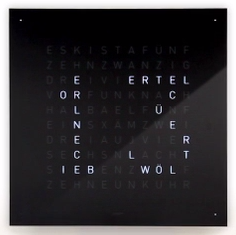
\includegraphics[width=0.8\columnwidth]{Abbildungen/Funktionen/Sekunden_01}

}

\begin{description}
\item[Taster 3] Anzeige der Raumtemperatur in $^\circ$C.
\end {description}
{
\centering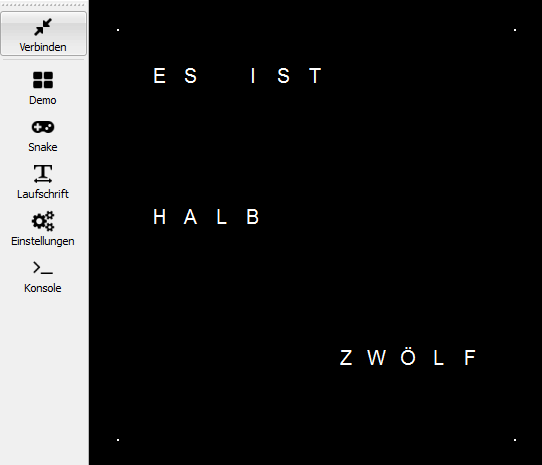
\includegraphics[width=0.8\columnwidth]{Abbildungen/Funktionen/Uhrzeit_01}

}

\begin{description}
\item[Taster 4] Einstellung der Helligkeit in 8 Stufen. Im letzten Modus ist die Uhr aus. Im ersten Modus wird die Helligheit automatisch über den Helligkeitssensor gesteuert.
\end {description}
 
\textbf{Helligkeit}

Über der Buchstabenmatrix befindet sich ein Helligkeitssensor. Mit Hilfe des Sensors passt sich die Helligkeit der LEDs automatisch an das Umgebungslicht an. So ist die Uhrzeit auch bei Nacht sehr angenehm zu lesen. Alternativ kann die Helligkeit manuell über den Taster vier in acht Stufen eingestellt werden.

\end{multicols}{2}